\documentclass[11pt]{article}

% load some asm stuff -
\usepackage{amssymb}
\usepackage{amsmath}
\usepackage{amsthm}
%\usepackage{palatino,lettrine}
\usepackage{fancyhdr}
\usepackage{epsfig}
%\usepackage[round,comma,sort]{natbib}
\usepackage{simplemargins}
\usepackage{setspace}
%\usepackage{boiboites}
\usepackage[margin=0pt,font=small,labelfont=bf]{caption}

\bibliographystyle{plos2009}

\makeatletter
\renewcommand{\@biblabel}[1]{\quad#1.}
\makeatother

% Set the size
%\textwidth = 6.75 in
%\textheight = 9.75 in
%\oddsidemargin = 0.0 in
%\evensidemargin = 0.0 in
%\topmargin = 0.01 in
%\headheight = 0.0 in
%\headsep = 0.25 in
%\parskip = 0.15in
\doublespace

\setallmargins{1in}

\newtheorem{example}{Example}[section]
\newtheorem{thm}{Theorem}[section]
\newtheorem{property}{Property}[section]

\theoremstyle{definition}
\newtheorem{defn}[thm]{Definition}

\usepackage{mdframed}
\definecolor{lgray}{rgb}{0.92,0.92,0.92}
\definecolor{lsalmon}{rgb}{1.0,0.63,0.48}

\makeatletter
\renewcommand\subsection{\@startsection
	{subsection}{2}{0mm}
	{-0.05in}
	{0.5\baselineskip}
	{\normalfont\normalsize\bfseries}}
\renewcommand\subsubsection{\@startsection
	{subsubsection}{2}{0mm}
	{-0.05in}
	{-0.5\baselineskip}
	{\normalfont\normalsize\bfseries}}
\renewcommand\paragraph{\@startsection
	{paragraph}{2}{0mm}
	{-0.05in}
	{-0.5\baselineskip}
	{\normalfont\normalsize\itshape}}
\makeatother
\linespread{1.2}

\fancypagestyle{proposal}{\fancyhf{}%
	\fancyhead[RO,LE]{\thepage}%
	\fancyhead[LO,RE]{CHEME 3130 Chemical Engineering Thermodynamics}%
	\renewcommand\headrulewidth{1pt}}
\pagestyle{proposal}

% Single space'd bib -
%\setlength\bibsep{0pt}

\renewcommand{\rmdefault}{phv}\renewcommand{\sfdefault}{phv}
%\newboxedtheorem[boxcolor=black, background=gray!5,titlebackground=orange!20,titleboxcolor = black]{color_box_example}{Example}{test}

% Change the number format in the ref list -
%\renewcommand{\bibnumfmt}[1]{#1.}

% Change Figure to Fig.
\renewcommand{\figurename}{Fig.}

%Joycelyn Chan, Joshua Lequieu, Michael Paull, Chidanand Balaji, Ryan Tasseff
%Our derivation follows closely the earlier development of Fredrickson \citep{Fredrickson:1976fk}.

% Begin ...
\begin{document}

%\begin{titlepage}
{\par\centering\textbf{\Large CHEME 3130: Analysis of Unit Paths in Thermodynamics}}
\vspace{0.2in}
{\par \centering \large{Jeffrey D. Varner$^{*}$}}
\vspace{0.05in}
{\par \centering \large{$^{*}$}Robert Frederick Smith School of Chemical and Biomolecular Engineering}
{\par \centering \large{Cornell University, Ithaca NY 14853}}
\vspace{0.1in}
{\par \centering \small{Copyright \copyright\ Jeffrey Varner 2017. All Rights Reserved.}}\\

%\end{titlepage}
\date{}
\thispagestyle{empty}

\setcounter{page}{1}

\begin{mdframed}[backgroundcolor=lgray]
\subsection*{Previously:}
\noindent We introduced generalized equations of state of the form:
\begin{equation}
	\mathcal{F}\left(T,P,v\right) = 0
\end{equation}
Common equations of state used in process calculations are the ideal gas law (for proof of concept calculations), cubic equations of state and generalized correlation models. The ideal gas law:
\begin{equation}
	Pv - RT = 0
\end{equation}is a hard-sphere model, molecules in the fluid occupy no volume and do not interact with another electrostatically.
For realistic process calculations, cubic equations of state are used:
\begin{equation}
	P = \frac{RT}{\left(v-b\right)}-\frac{a(T)}{\left(v+\epsilon b\right)\left(v+\sigma b\right)}
\end{equation}where $\epsilon$ and $\sigma$ are constants (the same for all substances), while
$a(T)$ and $b$ are substance specific, and be calculated in terms the critical temperature and pressure:
\begin{equation}
	a\left(T\right) = \Psi\left[\frac{\alpha\left(T_{r}\right)R^{2}T^{2}_{\mathrm{cr}}}{P_{\mathrm{cr}}}\right]\qquad
	b = \Omega\left[\frac{RT_{\mathrm{cr}}}{P_{\mathrm{cr}}}\right]
\end{equation}

\subsection*{Student outcomes:}
At the end of this lecture module, you will be able to:
\begin{itemize}
	\item[O$_1$]{Perform unit thermodynamic expansion and contraction operations using an ideal gas as a working fluid}
	\item[O$_2$]{Perform unit thermodynamic expansion and contraction operations using advanced cubic equations of state as the working fluid}
	\item[O$_3$]{Calculate the efficiency of hypothetical power generation cycles using the ideal gas as a working fluid}
\end{itemize}

\end{mdframed}

\clearpage

\section*{Introduction}
Just like complex chemical processes can be decomposed into many interconnected unit operations,
processes devised to convert heat to work e.g., steam engines, steam powered turbines or the internal combustion engine in your car
are also interconnected thermodynamic operations. These thermodynamic operations, called \textit{paths}, are composed of two types of physical operations, isothermal expansion (or contraction) and adiabatic expansion (or contraction). Let's start our discussion of these processes for \textit{closed} systems. Recall, that our general energy and material balances can be written in
differential form as:
\begin{eqnarray}\label{eqn:energy-balance-precursor-internal}
d\left(mu\right)\Bigr|_{sys} &=& \delta{Q}+\delta{W}+\sum_{s=1}^{\mathcal{S}}\nu_{s}u_{s}\delta{m}_{s} + \sum_{r=1}^{\mathcal{R}}\delta E_{r}\\\label{eqn:material-balance-precursor-internal}
dm &=& \sum_{s=1}^{\mathcal{S}}\nu_{s}\delta{m}_{s}
\end{eqnarray}where we have neglected changes in kinetic and potential energy in the system. For a closed system with no chemical reactions, our general differential balances reduce to:
\begin{equation}\label{eqn:first-law-differential}
dU = \delta{Q}+\delta{W}
\end{equation}and $\delta{m}_{s}$ = 0~$\forall{s}$. Eqn \eqref{eqn:first-law-differential} is the first-law of thermodynamics for a closed system with no chemical reactions,
where we have neglected changes in kinetic and potential energy. For each stage of our process, we'll apply the first law and then sum the work that is generated from the cycle.

\begin{figure*}[!ht]\centering
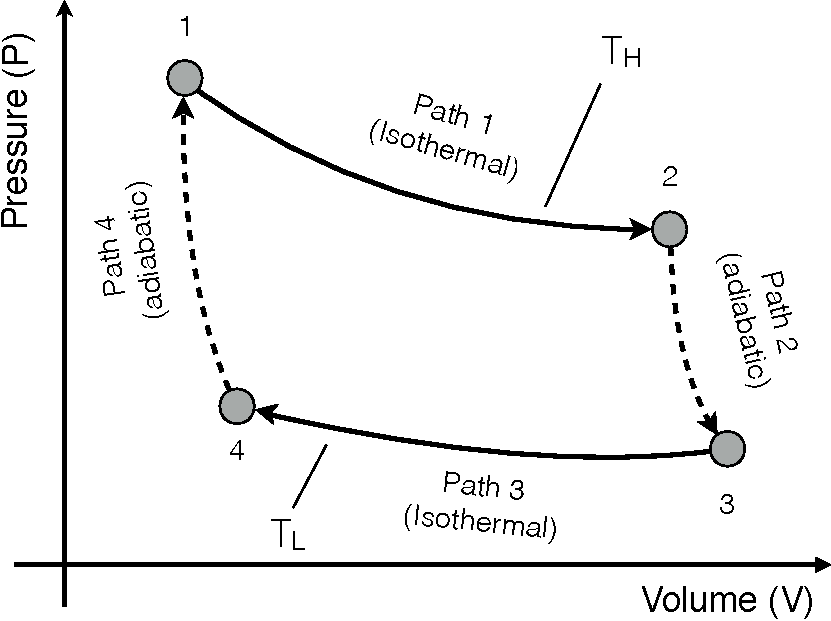
\includegraphics[width=0.6\textwidth]{./figs/CarnotCycle.pdf}
\caption{Schematic of the Carnot cycle. A working fluid is isothermally expanded from $\mathbb{P}_1$ to $\mathbb{P}_2$, and then adiabatically expanded from $\mathbb{P}_2$ to $\mathbb{P}_3$. The working fluid is then isothermally compressed from $\mathbb{P}_3$ to $\mathbb{P}_4$, and then adiabatically compressed from $\mathbb{P}_4$ back to the starting point $\mathbb{P}_1$.}\label{fig-carnot-cycle}
\end{figure*}

\subsection*{Carnot heat cycle for a closed system}
The Carnot cycle, named after the French engineer Sadi Carnot, is a hypothetical set of reversible expansion/compression operations
developed in 1824 as a model for the conversion of heat to work \cite{CARNOT_1824}.
The Carnot cycle involves two heat reservoirs, a hot reservoir maintained at $T_{H}$ and a cold reservoir maintained at $T_{L}$, along with two reversible isothermal operations,
and two reversible adibatic operations (Fig. \ref{fig-carnot-cycle}).
Starting from $\mathbb{P}_{1}$, a working fluid is
isothermally expanded from $\mathbb{P}_{1}$ to $\mathbb{P}_{2}$, and then adibatically expanded from $\mathbb{P}_{2}$ to $\mathbb{P}_{3}$.
The working fluid is then isothermally compressed from $\mathbb{P}_{3}$ to $\mathbb{P}_{4}$, and then adiabatically compressed from $\mathbb{P}_{4}$ back to the starting point $\mathbb{P}_{1}$.
If we assume the working fluid in the cycle is an ideal gas, whose internal energy is given by:
\begin{equation}\label{eqn:internal-energy-for-ideal-gas}
U = \frac{3}{2}Nk_{B}T
\end{equation} we can then derive the work generated by this cycle using the first-law for a closed system.

\begin{itemize}
\item{\textbf{Path~1}:~Isothermal expansion $\mathbb{P}_{1}\rightarrow\mathbb{P}_{2}$.
The first-law for path 1 is given by:
\begin{equation}
	dU_{1} = \delta{Q}_{1}+\delta{W}_{1}
\end{equation}or:
\begin{equation}
	dU_{1} = \delta{Q}_{1} - PdV
\end{equation}after substitution of the expansion work. We know (from statistical mechanics) that the internal energy of an ideal gas is given by Eqn \eqref{eqn:internal-energy-for-ideal-gas}.
Thus, the change in internal energy for path 1 is zero because $\mathbb{P}_{1}\rightarrow\mathbb{P}_{2}$ is isothermal:
\begin{equation}
	\Delta{U}_{\mathbb{P}_{1}\rightarrow\mathbb{P}_{2}} = \frac{3}{2}Nk_{B}\left(T_{H}-T_{H}\right) = 0
\end{equation}Constant internal energy along path 1 reduces the first law to:
\begin{equation}
	\delta{Q}_{1} = PdV
\end{equation}Subsituting the ideal-gas relationship for pressure $P = nRT_{H}/{V}$, and integrating between $\mathbb{P}_{1}\rightarrow\mathbb{P}_{2}$ gives an expression for the heat:
\begin{equation}
	Q_{1} = nRT_{H}\ln\left(\frac{V_{2}}{V_{1}}\right)
\end{equation}However, we know that
\begin{equation}
	\delta{Q}_{1} = -\delta{W}_{1}
\end{equation} thus the expansion work done in path 1 is given by:
\begin{equation}
	W_{1} = - nRT_{H}\ln\left(\frac{V_{2}}{V_{1}}\right)
\end{equation}}

\item{\textbf{Path~2}: Adiabatic expansion $\mathbb{P}_{2}\rightarrow\mathbb{P}_{3}$.
The first-law for path 2 is given by:
\begin{equation}
dU_{2} = \delta{Q}_{2} - PdV
\end{equation}after substitution of the expansion work. However, path 2 is \textit{adiabatic} which means $\delta{Q}_{2}$ = 0.
Thus, the first law for path 2 reduces to:
\begin{equation}
dU_{2} = -PdV
\end{equation}To estimate the work down by the adiabatic expansion, lets expand the internal energy:
\begin{equation}
		dU = \left(\frac{\partial{U}}{\partial{T}}\right)_{V}dT + \left(\frac{\partial{U}}{\partial{V}}\right)_{T}dV
\end{equation}which gives:
\begin{equation}
\left(\frac{\partial{U}}{\partial{T}}\right)_{V}dT + \left(\frac{\partial{U}}{\partial{V}}\right)_{T}dV = -PdV
\end{equation}or after collecting like differential terms:
\begin{equation}\label{eqn:general-adibatic-expansion}
\left(\frac{\partial{U}}{\partial{T}}\right)_{V}dT = -\left[ \left(\frac{\partial{U}}{\partial{V}}\right)_{T} + P\right]dV
\end{equation}Eqn \eqref{eqn:general-adibatic-expansion} can be applied for a general working fluid; however, we are analyzing the
Carnot cycle for an ideal gas. Thus, we can simply Eqn \eqref{eqn:general-adibatic-expansion} by first realizing that:
\begin{equation}
\left(\frac{\partial{U}}{\partial{V}}\right)_{T} = 0
\end{equation}and second:
\begin{equation}
C_{V} = \left(\frac{\partial{U}}{\partial{T}}\right)_{V}
\end{equation}which gives:
\begin{equation}
C_{V}dT = -PdV
\end{equation}or:
\begin{equation}\label{eqn:work-heat-capacity-path-2}
\delta{W}_{2} = C_{V}dT
\end{equation}
Eqn \eqref{eqn:work-heat-capacity-path-2} says that we can directly relate the work done to the temperature change in the working fluid of the system.
Integrating both sides of Eqn \eqref{eqn:work-heat-capacity-path-2} gives the work done by path 2:
\begin{equation}
W_{2} = \int_{T_{H}}^{T_{L}}C_{V}dT
\end{equation}or:
\begin{equation}
W_{2} = C_{V}\left(T_{L} - T_{H}\right)
\end{equation}}

\item{\textbf{Path~3}:~Isothermal compression $\mathbb{P}_{3}\rightarrow\mathbb{P}_{4}$.
Following the derivation for path 1, the work generated by isothermal expansion from $\mathbb{P}_{3}\rightarrow\mathbb{P}_{4}$ is given by:
\begin{equation}
W_{3} = - nRT_{L}\ln\left(\frac{V_{4}}{V_{3}}\right)
\end{equation}}

\item{\textbf{Path~4}:~Adiabatic compression $\mathbb{P}_{4}\rightarrow\mathbb{P}_{1}$.
Following the derivation of path 2, the work generated by adibatic expansion from $\mathbb{P}_{4}\rightarrow\mathbb{P}_{1}$ is given by:
\begin{equation}
W_{4} = C_{V}\left(T_{H} - T_{L}\right)
\end{equation}}
\end{itemize}

\subsection*{Efficiency of the Carnot cycle}
The efficiency of a Carnot cycle, denoted by the symbol $\eta$, is defined as the net work done by the system, divided by the net input heat:
\begin{equation}
\eta = -\frac{W_{net}}{Q_{in}}
\end{equation}Using our first law results, we can put the efficiency in terms of the two operating parameters we control, the temperature of the
hold and cold reservoirs:
\begin{equation}\label{eqn:carnot-efficinecy}
\eta = 1 - \frac{T_{L}}{T_{H}}
\end{equation}We can increase the efficiency by allowing $T_{H}\rightarrow\infty$ or by having a small value for $T_{L}$.
As we shall see, the Carnot cycle is the \textit{most} efficient cycle for converting heat to work.
However, unfortunately Carnot is imaginary but it can serve as a useful model system to measure real results against.

\subsubsection*{Change in a state function for a cyclic process}
Beyond its efficiency, one of the other interesting things about Carnot is that it nicely demonstrates one of the central properties of \textit{state functions}:
\begin{equation}
dU = \sum_{j=\mathbb{P}_{1}}^{\left\{\mathbb{P}_{j}:\mathbb{P}_{j}\neq\mathbb{P}_{1}\right\}}dU_j = 0
\end{equation}The net change in a state function, such as internal energy, temperature, pressure or volume (irrespective of the working fluid) is zero around a closed path.
This has important consequences later, and is easy to see from our first law analysis of the Carnot cycle: where
\begin{equation}
dU = dU_{1}+dU_{2}+dU_{3}+dU_{4}
\end{equation}If we ignore the fact that our working fluid is an ideal gas (assume its some arbitrary fluid), we simply need to integrate the $dU$ expression around the
path:
\begin{equation}
\int_{\mathbb{P}_{1}}^{\mathbb{P}_{1}}dU = \int_{\mathbb{P}_{1}}^{\mathbb{P}_{2}}dU_{1}+\int_{\mathbb{P}_{2}}^{\mathbb{P}_{3}}dU_{2}+\int_{\mathbb{P}_{3}}^{\mathbb{P}_{4}}dU_{3}+\int_{\mathbb{P}_{4}}^{\mathbb{P}_{1}}dU_{4}
\end{equation}or:
\begin{equation}
U_{1} - U_{1} = \left(U_{2} - U_{1}\right) + \left(U_{3} - U_{2}\right) + \left(U_{4} - U_{3}\right) + \left(U_{1} - U_{4}\right) = 0
\end{equation}Even if we consider an ideal gas, we know that both $dU_{1}$ = 0 and $dU_{3}$ = 0 which gives:
\begin{equation}
dU  = dU_{2} + dU_{4}
\end{equation}or:
\begin{equation}
dU = C_{V}dT\Bigr|_{\mathbb{P}_{2}\rightarrow\mathbb{P}_{3}}+C_{V}dT\Bigr|_{\mathbb{P}_{4}\rightarrow\mathbb{P}_{1}}
\end{equation}Integrating both sides of the differential internal energy equation gives:
\begin{equation}
\Delta{U} = C_{V}\int_{T_{H}}^{T_{L}}dT+C_{V}\int_{T_{L}}^{T_{H}}dT
\end{equation}or:
\begin{equation}
\Delta{U} = C_{V}\left[\left(T_{H} - T_{L}\right)+\left(T_{L} - T_{H}\right)\right] = 0
\end{equation}
Interestingly, non-state variables, such as heat and work, are \textit{not} conserved along a closed path. To see that, lets compute the
net work done by the cycle:
\begin{equation}
\delta{W}_{net} = \sum_{j=\mathbb{P}_{1}}^{\left\{\mathbb{P}\right\}}\delta{W}_j\neq 0
\end{equation}or after integration and substitution of work definitions:
\begin{equation}
W_{net} = - nRT_{H}\ln\left(\frac{V_{2}}{V_{1}}\right) + C_{V}\left(T_{L} - T_{H}\right) - nRT_{L}\ln\left(\frac{V_{4}}{V_{3}}\right) + C_{V}\left(T_{H} - T_{L}\right)
\end{equation}which reduces to:
\begin{equation}
W_{net} = - nRT_{H}\ln\left(\frac{V_{2}}{V_{1}}\right) - nRT_{L}\ln\left(\frac{V_{4}}{V_{3}}\right) \neq{0}
\end{equation}




\bibliography{References}

\end{document}
